% Template for EUSIPCO 2015 paper; to be used with:
%          spconf.sty  - LaTeX style file, and
%          IEEEbib.bst - IEEE bibliography style file.
% --------------------------------------------------------------------------
\documentclass[a4paper]{article}
\usepackage{spconf,amsmath,graphicx,cite}

% Example definitions.
% --------------------
\def\x{{\mathbf x}}
\def\L{{\cal L}}

% Title.
% ------
\title{AUTHOR GUIDELINES FOR EUSIPCO 2015 PROCEEDINGS MANUSCRIPTS}
%
% Single address.
% ---------------
\name{Author(s) Name(s)\thanks{Thanks to XYZ agency for funding.}}
\address{Author Affiliation(s)}
%
% For example:
% ------------
%\address{School\\
%	Department\\
%	Address}
%
% Two addresses (uncomment and modify for two-address case).
% ----------------------------------------------------------
%\twoauthors
%  {A. Author-one, B. Author-two\sthanks{Thanks to XYZ agency for funding.}}
%	{School A-B\\
%	Department A-B\\
%	Address A-B}
%  {C. Author-three, D. Author-four\sthanks{The fourth author performed the work
%	while at ...}}
%	{School C-D\\
%	Department C-D\\
%	Address C-D}
%
% Multiple author/addresses combination (use only in particular cases).
% ---------------------------------------------------------------------
%\name{A. Author-one$^*$, B. Author-two$^*$$^\dagger$, C. Author-three$^\dagger$, D. Author-four$^\ddagger$ %
%	\thanks{General thanks/acknowledgment}%
%	\thanks{$^*$ Thanks/acknowledgments for authors marked with *}%
%	\thanks{$^\dagger$ Thanks/acknowledgments for authors marked with $\dagger$}%
%	\thanks{$^\ddagger$ Thanks/acknowledgments for authors marked with $\ddagger$}%
%}
%\address{%
%    \tabular{c}
%		$^*$ Institute ABC\\
%		Group Group ABC\\
%		Address ABC
%	\endtabular
%	\hskip 0.5in
%    \tabular{c}
%		$^\dagger$ School DEF\\
%		Department DEF\\
%		Address DEF
%	\endtabular
%	\hskip 0.5in
%    \tabular{c}
%		$^\ddagger$ Company GHI\\
%		Department GHI\\
%		Address GHI
%	\endtabular
%}
%
% The symbol order for multiple author combination is:
%  $^*$, $^\dagger$, $^\ddagger$, $^\mathsection$, $^\mathparagraph$, $^\|$,
%  $^{**}$, $^{\dagger\dagger}$, $^{\ddagger\ddagger}$, ...
%
%
% Alternative multiple author/addresses combination (use only in particular cases).
% ---------------------------------------------------------------------------------
%\name{A. Author-one$^*$, B. Author-two$^*$$^\dagger$, C. Author-three$^\dagger$, D. Author-four$^\ddagger$ %
%	\thanks{General thanks/acknowledgment}%
%	\thanks{$^*$ Thanks/acknowledgments for authors marked with *}%
%	\thanks{$^\dagger$ Thanks/acknowledgments for authors marked with $\dagger$}%
%	\thanks{$^\ddagger$ Thanks/acknowledgments for authors marked with $\ddagger$}%
%}
%\address{%
%	$^*$ Institute ABC, Group Group ABC, Address ABC\\
%	$^\dagger$ School DEF, Department DEF, Address DEF\\
%	$^\ddagger$ Company GHI, Department GHI, Address GHI\\
%}
%
% The symbol order for multiple author combination is:
%  $^*$, $^\dagger$, $^\ddagger$, $^\mathsection$, $^\mathparagraph$, $^\|$,
%  $^{**}$, $^{\dagger\dagger}$, $^{\ddagger\ddagger}$, ...
%
\begin{document}

%
\maketitle
%
\begin{abstract}
The abstract should appear at the top of the left-hand column of text, about
0.5 inch (12 mm) below the title area and it should be no more than 3.125 inches (80 mm) in
length.  Leave a 0.5 inch (12 mm) space between the end of the abstract and the
beginning of the main text.  The abstract should must contain 100 to 150
words, and must be identical to the abstract text submitted electronically
along with the paper cover sheet.  All manuscripts must be in English.
\end{abstract}
%
\begin{keywords}
One, two, three, four, five
\end{keywords}
%
\section{Introduction}
\label{sec:intro}

These guidelines include complete descriptions of the fonts, spacing, and
related information for producing your proceedings manuscripts. Please follow
them.

First of all, here is some general information about the paper preparation, submission, and review process.

\begin{itemize}
  \item Papers submitted to EUSIPCO 2015 must describe original, unpublished work. The papers must contain a complete description of the ideas presented and applicable research results.
  \item Papers must conform to the format and style specified in this document. The deadline for the submission of full papers is February 13, 2015. The maximum paper length including figures and references is five (5) pages.
  \item Based on comments from the reviewers, it will be possible to make changes to your paper before it is submitted in its final, camera-ready form by June 19, 2015.
  \item All submitted papers that conform to the style instructions specified in this document will be reviewed by anonymous reviewers, selected by the conference committee for their demonstrated knowledge of particular topics. The review process will be carried online and the results of the reviewing will be posted on this web-site, and authors will also be notified of the review results by email by May 22, 2015.
  \item Accepted papers will be published in the EUSIPCO 2015 Proceedings (distributed to conference attendees and accessible on the IEEE web-site).
  \item At least one author of each accepted paper must register for the conference at full registration rate no later than June 19, 2015 (the EUSIPCO 2015 registration site will be opened in due time).
\end{itemize}

\section{Formatting your paper}
\label{sec:format}

Paper size should be set to A4 (210 mm $\times$ 297 mm). Letter (8.5 $\times$ 11-inch) is also acceptable, but in that case set the top and left margins as specified below. All printable material, including text, figures and tables, must be kept within a print area of 7 inches (178~mm) wide by 9 inches (229~mm) high. Do not write anything outside the print area. The top margin must be 1 inch (25~mm), except for the title page, and the left margin must be 0.75 inch (19~mm).  All text must be in a two-column format. Columns are to be 3.39 inches (86 mm) wide, with a 0.24 inch (6~mm) space between them. Text must be fully justified. If the last page of your paper is only partially filled, arrange the columns so that they are evenly balanced, rather than having one long column.

%In LaTeX, to start a new column (but not a new page) and help balance the last-page column lengths, you can use the command ``$\backslash$pagebreak'', as demonstrated near the end of the LaTeX source for this template.

\section{PAGE TITLE SECTION}
\label{sec:pagestyle}

The paper title (on the first page) should begin 1.38 inches (35 mm) from the
top edge of the page, centered, completely capitalized, and in Times 14-point,
boldface type. The authors' name(s) and affiliation(s) appear below the title
in capital and lower case letters. Authors' name(s) should be in italics.
Papers with multiple authors and affiliations may require two or more lines for this information.

\section{TYPE-STYLE AND FONTS}
\label{sec:typestyle}

To achieve high rendering quality in the proceedings and to give them a uniform look, a Times-Roman font should be used. The font size should be no smaller than 10-point throughout the main body of the text and the font color must be black. TrueType or Postscript Type 1 fonts are preferred.

Please do not use double-space in your paper. The first paragraph in each section should not be indented, but all following paragraphs within the section should be indented as these paragraphs demonstrate.


\section{MAJOR HEADINGS}
\label{sec:majhead}

Major headings, \textit{e.g.}, ``\textbf{1. INTRODUCTION}'', should appear in all capital
letters, bold face if possible, centered in the column, with one blank line
before, and one blank line after. Use a period (``.'') after the heading number,
not a colon.

\subsection{Subheadings}
\label{ssec:subhead}

Subheadings should appear in lower case (initial word capitalized) in
boldface.  They should start at the left margin on a separate line.

\subsubsection{Sub-subheadings}
\label{sssec:subsubhead}
Sub-subheadings, as in this paragraph, are discouraged. However, if you
must use them, they should appear in lower case (initial word
capitalized) in italics. They should start at the left margin on a separate line.


\section{PAGE NUMBERING}
\label{sec:page}

Please do {\bf not} paginate your paper.  Page numbers, session numbers, and
conference identification will be inserted when the paper is included in the
proceedings.

\section{Figures and Tables}
\label{sec:illust}

Figures and tables must appear within the designated margins.  They may span the two columns.  If possible, position figures and tables at the top of columns, rather than in the middle or at the bottom. Caption and number every figure and every table using Times 9-point type, as shown in Figure~\ref{fig:res} and in Table~\ref{tab:res}. All halftone illustrations must be clear black and white prints.  If you use color, make sure that the color figures are clear when printed on a black-only printer.

Since there are many ways, often incompatible, of including images (e.g., with
experimental results) in a LaTeX document, Figure~\ref{fig:res} shows an example of how to do
this.

% Below is an example of how to insert images. Delete the ``\vspace'' line,
% uncomment the preceding line ``\centerline...'' and replace ``imageX.eps''
% with a suitable PostScript file name.
% -------------------------------------------------------------------------
\begin{figure}

\begin{minipage}[b]{1.0\linewidth}
  \centering
  \centerline{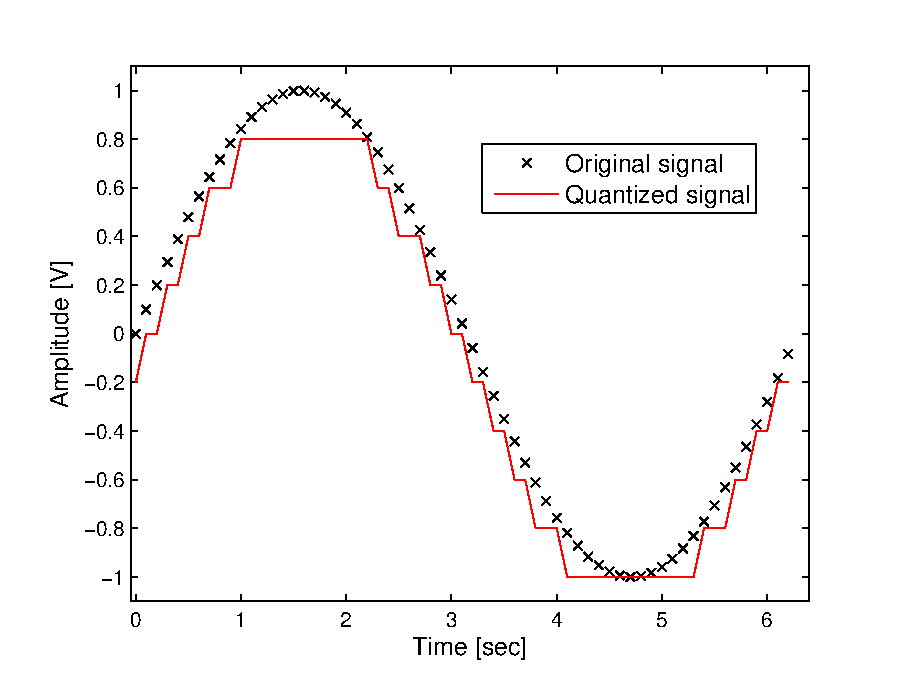
\includegraphics[width=4.9cm]{image1.eps}}
%  \vspace{2.0cm}
  \small\centerline{(a) Result 1}\medskip
\end{minipage}
%
\begin{minipage}[b]{.48\linewidth}
  \centering
  \centerline{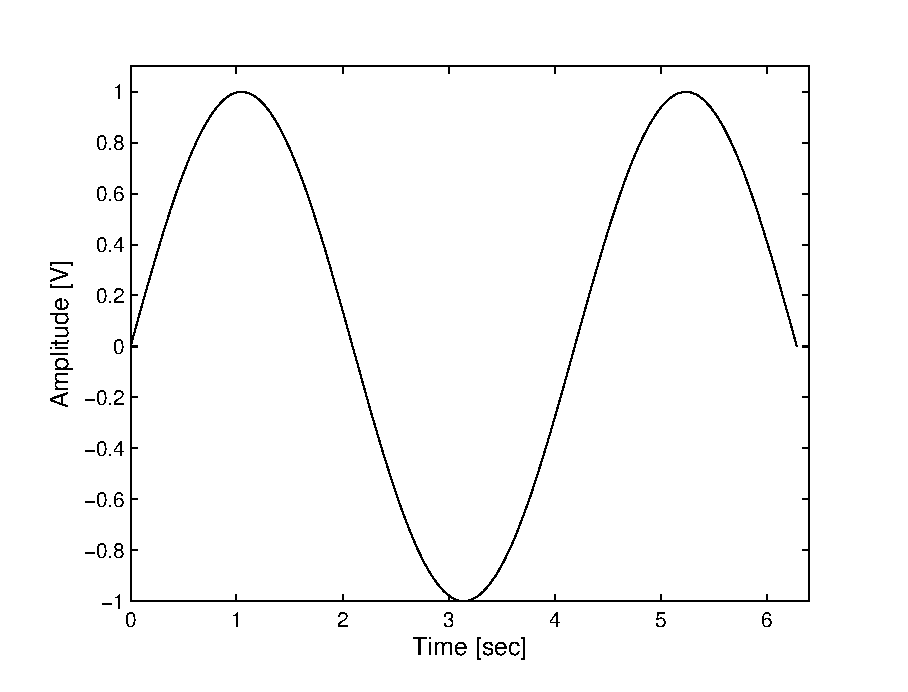
\includegraphics[width=4.1cm]{image2.eps}}
%  \vspace{1.5cm}
  \small\centerline{(b) Result 2}\medskip
\end{minipage}
\hfill
\begin{minipage}[b]{0.48\linewidth}
  \centering
  \centerline{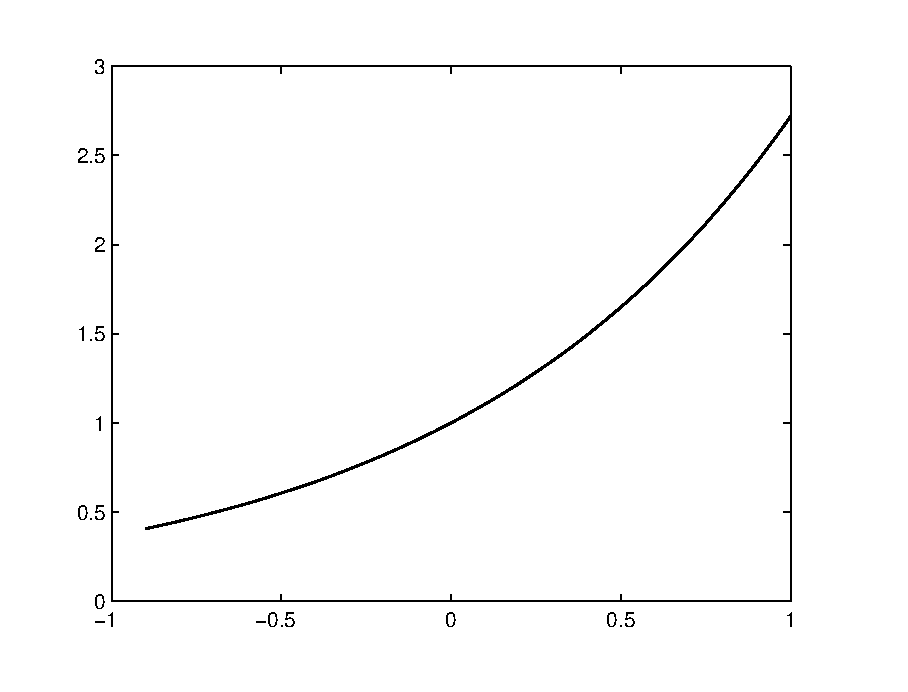
\includegraphics[width=4.1cm]{image3.eps}}
%  \vspace{1.5cm}
  \small\centerline{(c) Result 3}\medskip
\end{minipage}
%
\vspace*{-0.3cm}
\caption{Example of placing a figure with experimental results.}
\label{fig:res}
%
\end{figure}


\section{Equations}
Equations should be centered within the respective column as shown in~\eqref{eq:capacity}:
%
\begin{equation}
C = \frac{1}{2}\log_2{\left(1+\frac{P}{\sigma^2}\right)}.
\label{eq:capacity}
\end{equation}
%

Punctuate all equations and number those referenced in the text. When referencing an equation, use ``\eqref{eq:capacity}'' instead of ``eq.~\eqref{eq:capacity}'' or ``equation~\eqref{eq:capacity}'', except at the beginning of a sentence: ``Equation~\eqref{eq:capacity} is...''. Math fonts are allowed to be used in the equations (\textit{e.g.}, Cambria or Computer Modern), but their size should be uniform and similar to the font size used along the text.


\section{FOOTNOTES}
\label{sec:foot}

Use footnotes sparingly (or not at all!) and place them at the bottom of the
column on the page on which they are referenced. Use Times 9-point type,
single-spaced. To help your readers, avoid using footnotes altogether and
include necessary peripheral observations in the text (within parentheses, if
you prefer, as in this sentence).


\begin{table}
\small
\begin{center}
\renewcommand{\arraystretch}{1.2}
\begin{tabular}{lcc}
\hline
\textbf{Experiment}    & \textbf{Result 1} & \textbf{Result 2} \\
\hline
First experiment  & 10 & 20 \\
Second experiment & 20 & 35 \\
\hline
\end{tabular}
\end{center}
\vspace*{-0.3cm}
\caption{Example of a table.}
\label{tab:res}
\end{table}


\section{REFERENCES}
\label{sec:ref}

List and number all bibliographical references at the end of the paper.  The references should be numbered in order of appearance in the document.  When referring to them in the text, type the corresponding reference number in square brackets as shown at the end of this sentence \cite{A1}. For multiple citations at once, separate reference numbers by commas inside the square brackets as in~\cite{A1,P1}, or use the compressed format as in~\cite{A1,P1,B1}.

\section{PAPER SUBMISSION}
\label{sec:submission}

Papers must be submitted through the EDAS system. When entering the electronic submission system for the first time, you will have to ``sign up'' to get a user ID and password. \textbf{Accepted file format is PDF only.}

All fonts used must be embedded in the PDF file. However, Asian fonts must not be used nor embedded. Documents that do not print correctly on a Post-Script printer cannot be accepted. (When printing the PDF file, make sure that the ``shrink to fit'' box is not checked!) Providing a correct and printable PDF file is entirely under the authors' responsibility. If the paper is not printable, the review procedure will not be initiated.

In addition to uploading their paper, authors are required to provide the following information (ASCII text) via the sub-mission web site:

\begin{itemize}
  \item Appropriate track,
  \item Paper title (in Title Case),
  \item Up to 5 Keywords for the paper,
  \item Affiliations, email addresses, and mailing addresses for each author,
  \item Paper abstract, in ASCII text format (for copying and pasting into web page form), with 100 to 150 words, and
  \item Up to 10 topic areas for the paper.
\end{itemize}

After you submit the information on the paper title, abstract text, review category, and author contact information, the system will display a page ({\it registering paper}) with the data that you entered so that you may verify its accuracy. If you need to change the data to fix a mistake, you may use the back button on your browser to return to the information entry form. After approval of your data, you may choose your document file for upload at the bottom (``upload'' link) of the ``registering paper'' page. Your browser will upload your file to the EUSIPCO 2015 server. At the end of a successful upload, you will see a confirmation page displaying the paper number that is assigned to you, the dimension of the paper and the uploading date. An e-mail message will be sent to the authors' email addresses to confirm that the file has indeed been registered and uploaded.

\vfill\pagebreak
\section{REVIEW PROCESS}
\label{sec:review}

A committee of reviewers selected by the conference Technical Program Committee (TPC) will review the submitted papers and rate them according to quality, relevance, and correctness. The conference TPC will use these reviews to determine which papers will be accepted for presentation in the conference, and in which form (oral/poster). The result of the technical committee's decision will be communicated to the submitting authors by email, along with reviewer comments.

% To start a new column (but not a new page) and help balance the last-page
% column length use \vfill\pagebreak.
% -------------------------------------------------------------------------


\section{REGISTER FOR THE CONFERENCE}
\label{sec:reg}
Be sure that at least one author registers to attend the conference using the online registration system available through conference web-site: http://www.eusipco2015.org/. A full registration by (at least) one of the paper's authors is required for each accepted paper. The payment must be received by the deadline of the author registration. Papers that have not been associated with a full registration by one of the paper's authors will not be published in the EUSIPCO 2015 proceedings. If you are an author, \textbf{you may associate with your full registration no more than three papers of which you are (co)author}.


\section{IMPORTANT DATES}
\label{sec:dates}

\begin{center}	
\begin{tabular}{ll}
Paper submission deadline:    & February 13, 2015 \\
Notification of acceptance:   & May 22, 2015   \\
Author registration deadline: & June 19, 2015 \\
Camera-ready final paper due: & June 19, 2015
\end{tabular}
\end{center}

% References should be produced using the bibtex program from suitable
% BiBTeX files (here: strings, refs, manuals). The IEEEbib.bst bibliography
% style file from IEEE produces unsorted bibliography list.
% -------------------------------------------------------------------------
\bibliographystyle{IEEEbib}
\bibliography{strings,refs}

\end{document}
